\section{Hermite Algorithm for Periodicity Detection (\HAPD)}\label{sec:hapd_algorithm}

This section presents the Hermite Algorithm for Periodicity Detection (HAPD), a non-subtractive approach that leverages projective geometry to identify periodicity in cubic irrationals. The algorithm builds upon the theoretical foundations established in Sections~\ref{sec:galois_theory} and \ref{sec:matrix_approach}.

\begin{figure}[ht]
\centering
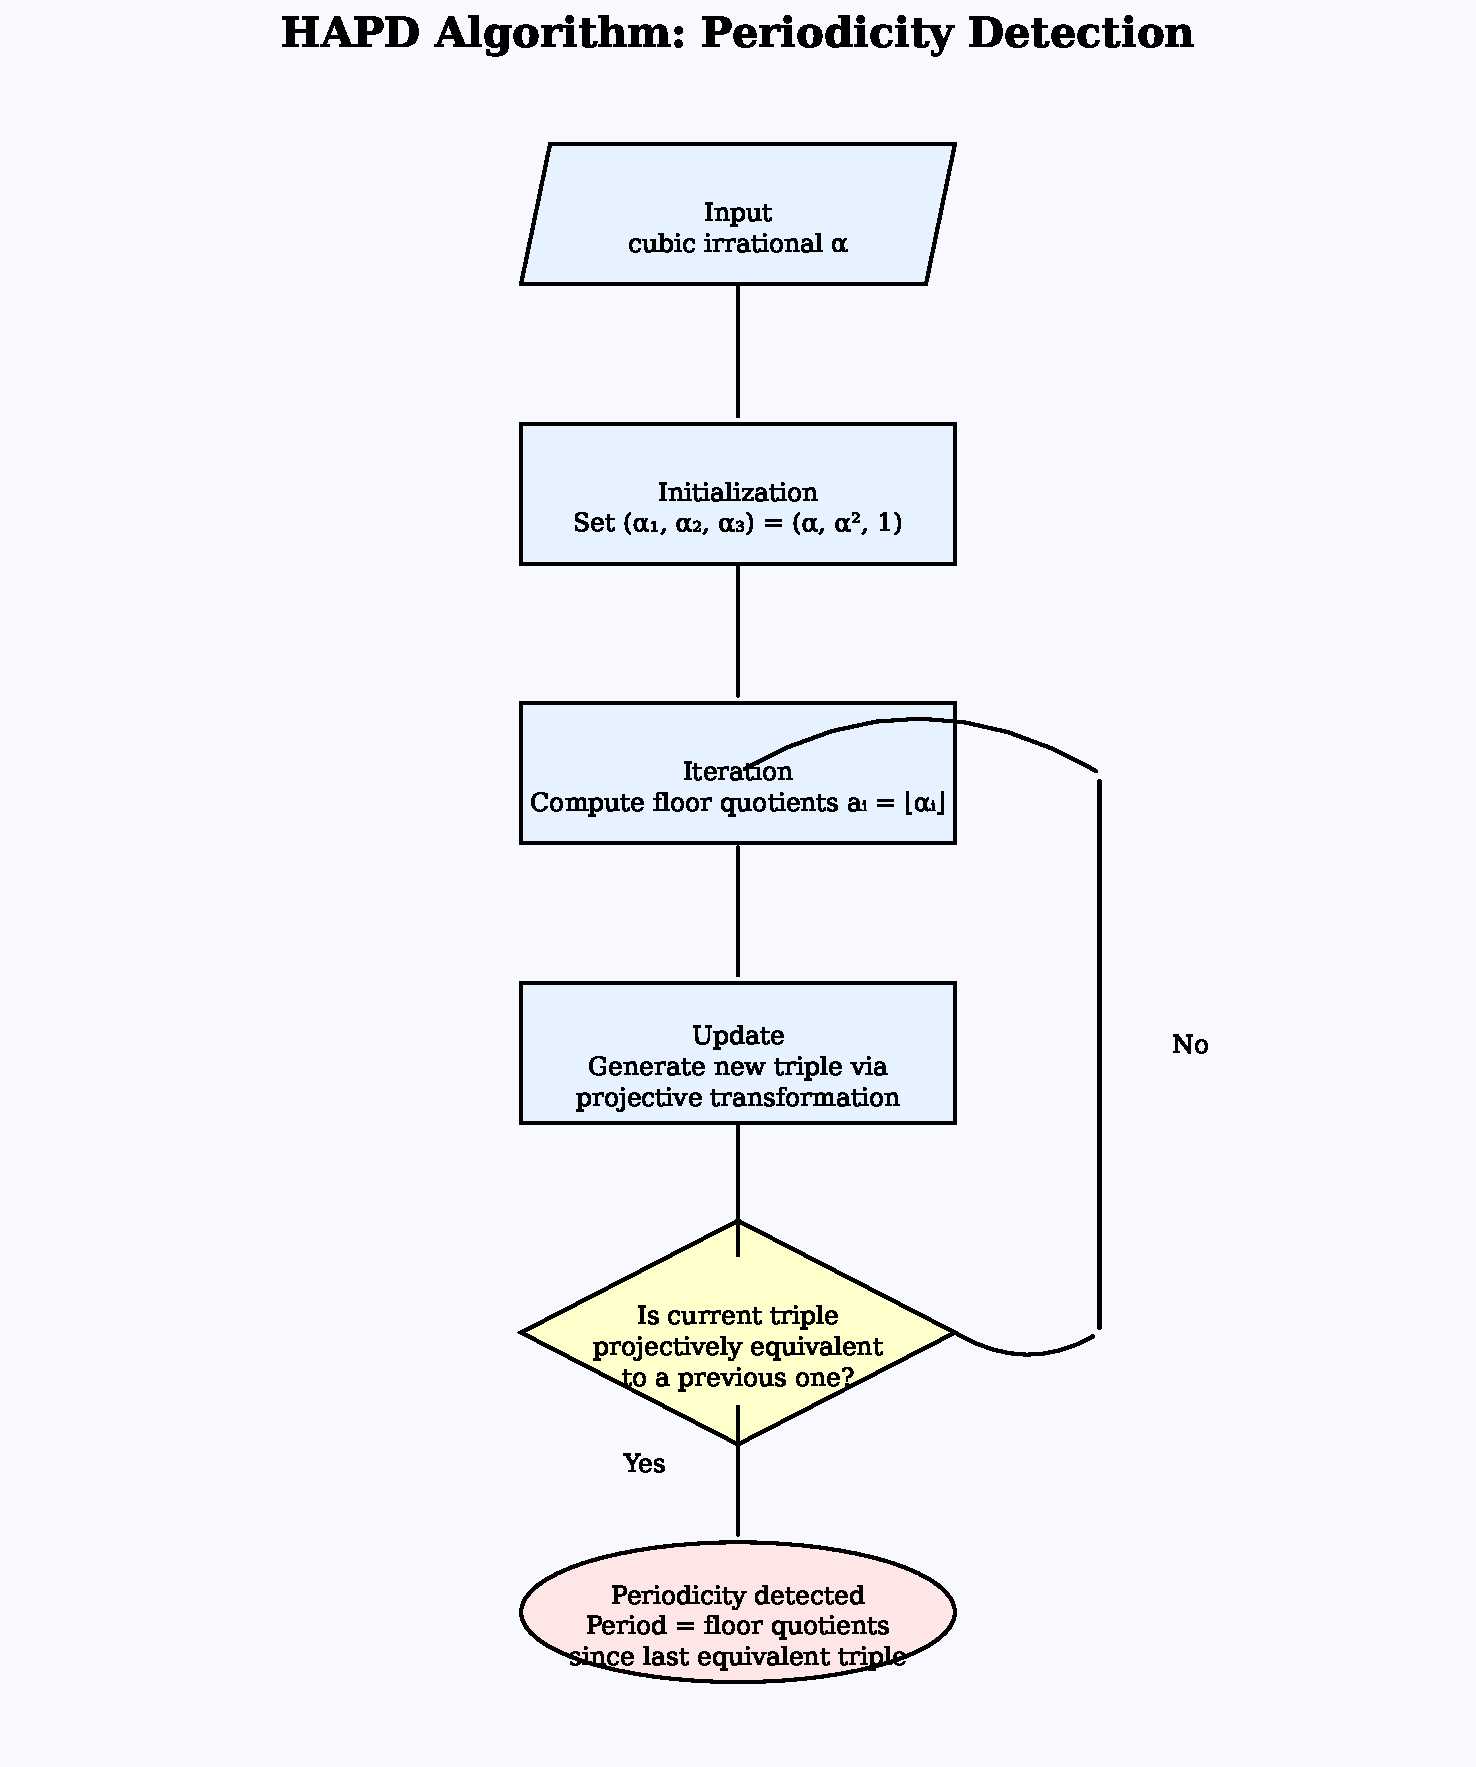
\includegraphics[width=0.8\textwidth]{figures/output/hapd_algorithm_flowchart.pdf}
\caption{Flowchart of the Hermite Algorithm for Periodicity Detection (HAPD) showing the process of identifying periodicity in the continued fraction expansion of cubic irrationals.}
\label{fig:hapd_flowchart}
\end{figure}

\begin{figure}[ht]
\centering
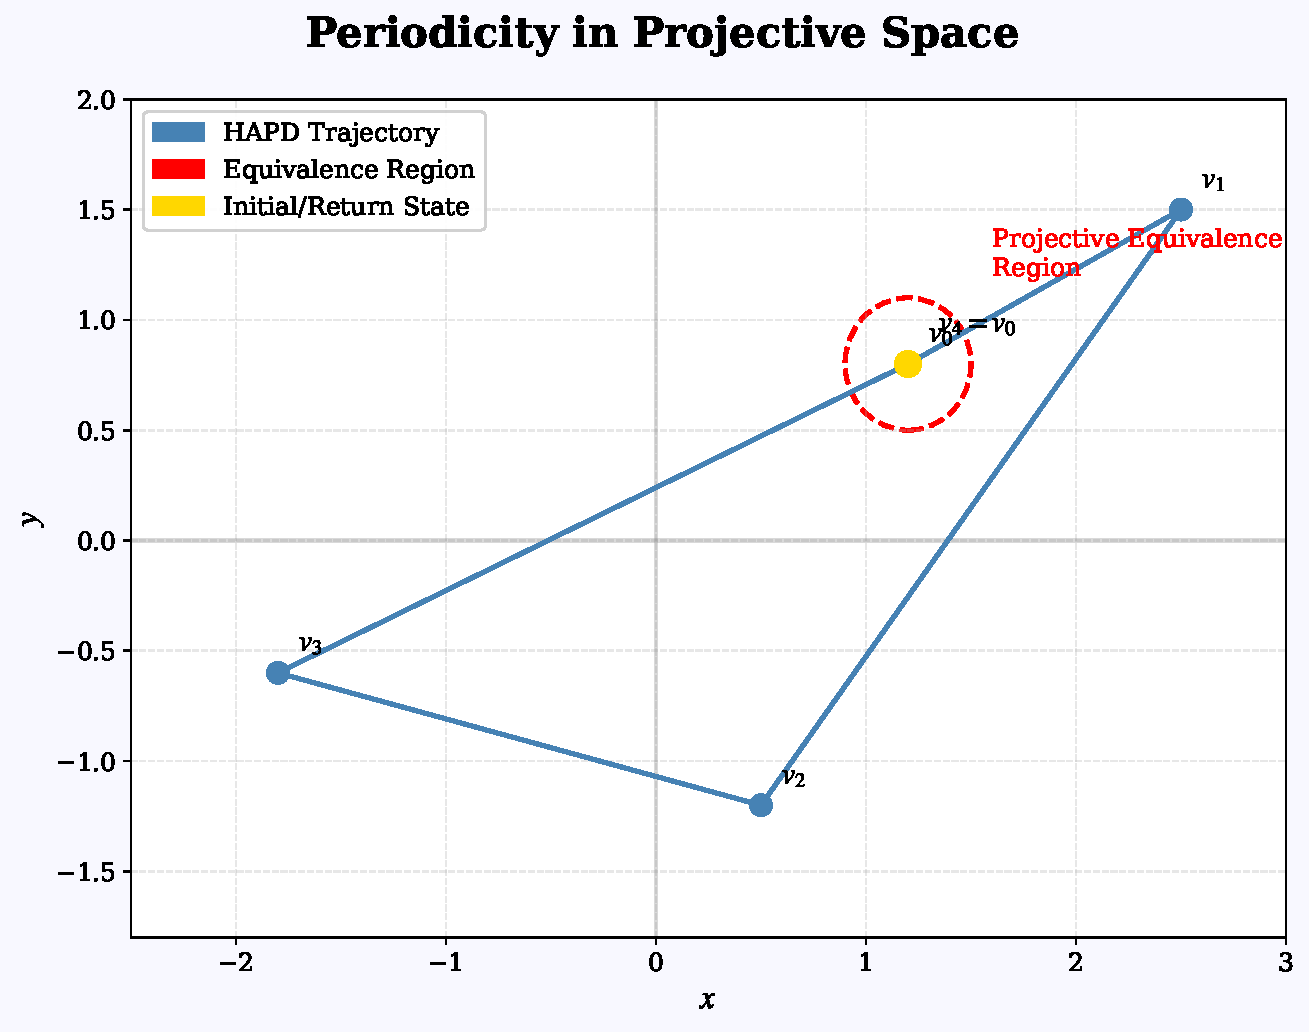
\includegraphics[width=0.85\textwidth]{figures/output/projective_periodicity_visualization.pdf}
\caption{Visualization of the periodicity detection in projective space. Points $v_0$ through $v_3$ represent projective triples generated by the HAPD algorithm. The point $v_4$ returning to the projective equivalence region around $v_0$ confirms periodicity.}
\label{fig:projective_visualization}
\end{figure}

\begin{figure}[ht]
\centering
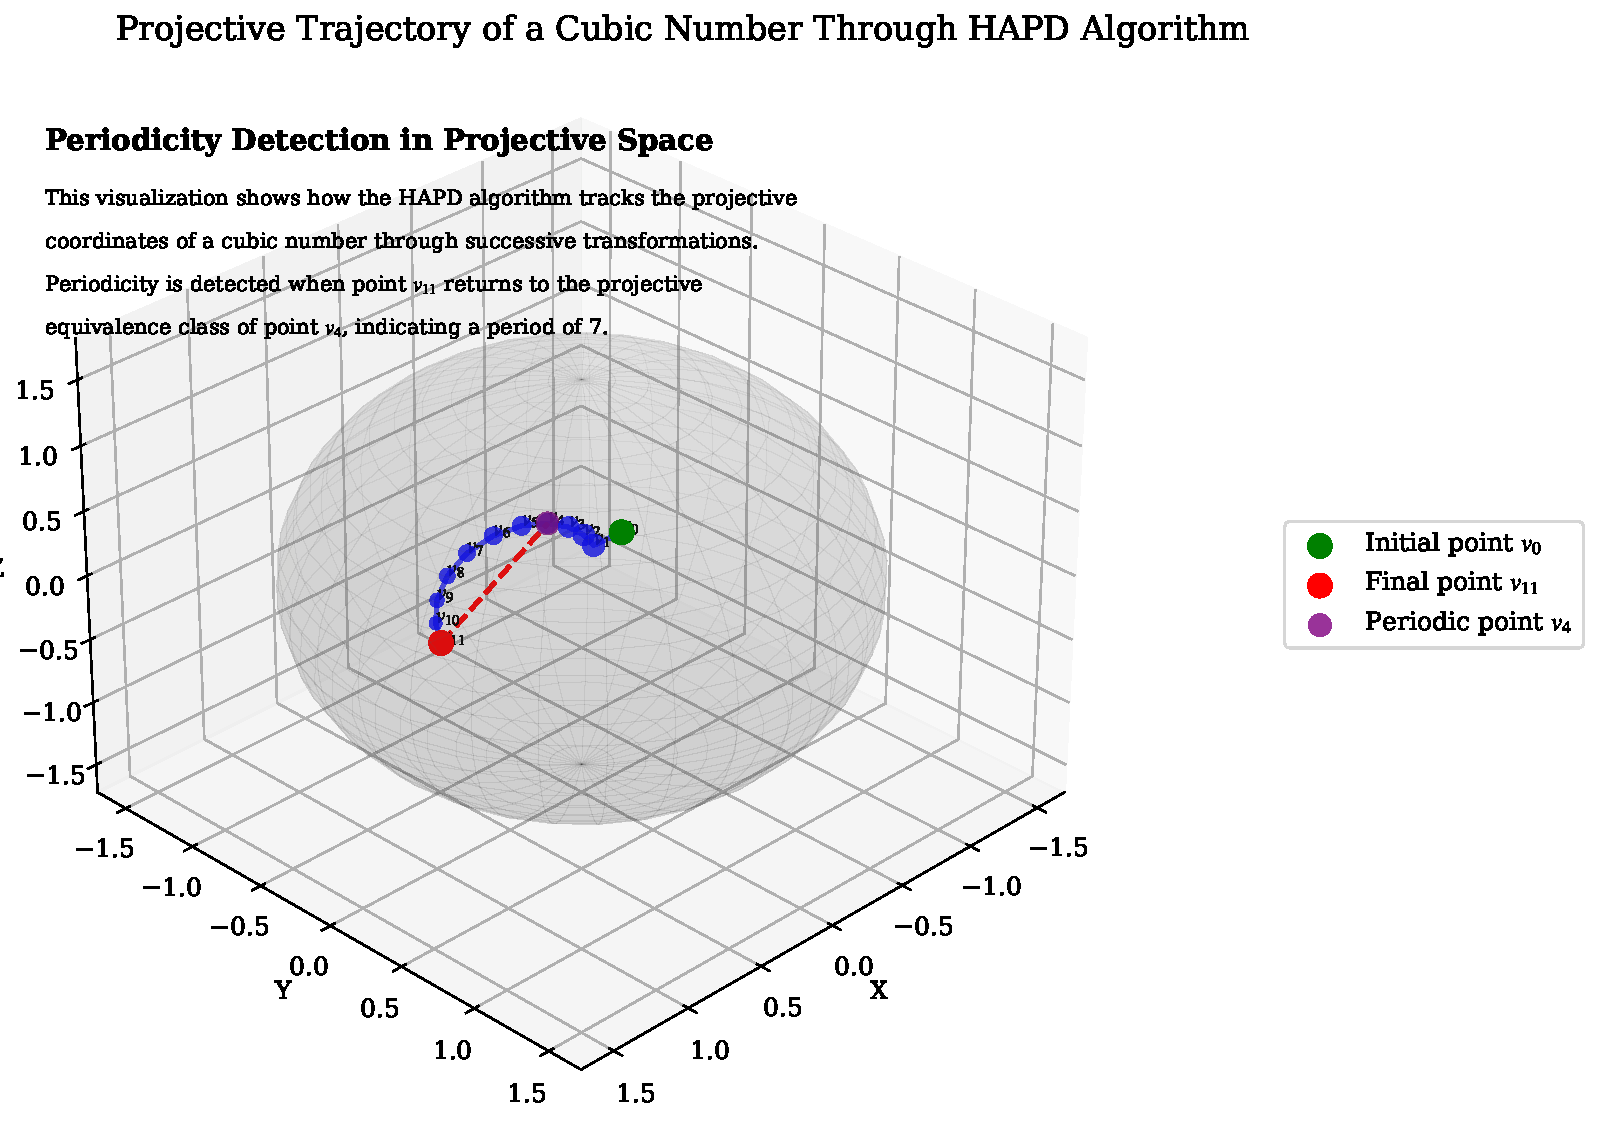
\includegraphics[width=0.9\textwidth]{../figures/output/projective_trajectory_visualization.pdf}
\caption{Visualization of the projective trajectory for $\sqrt[3]{2}$ through HAPD algorithm iterations. The blue line shows the path of successive projective triples, with points $v_0$ through $v_{11}$ representing algorithm iterations. Periodicity is detected when point $v_{11}$ returns to the projective equivalence class of point $v_4$ (connected by the red dashed line), establishing a period of 7.}
\label{fig:projective_trajectory}
\end{figure}

\subsection{Theoretical Foundation}

The HAPD algorithm is based on the insight that projective transformations offer a natural framework for detecting periodicity in cubic irrationals. By operating in projective space $\mathbb{P}^2$, the algorithm bypasses many of the complications that arise when working with traditional continued fractions and their multidimensional extensions.

\begin{definition}[HAPD Transformation]
For a point $\mathbf{p} = (x, y, z) \in \mathbb{P}^2$, define the HAPD transformation $T: \mathbb{P}^2 \rightarrow \mathbb{P}^2$ as:
\begin{equation}
T(\mathbf{p}) = 
\begin{pmatrix}
a_{11} & a_{12} & a_{13} \\
a_{21} & a_{22} & a_{23} \\
a_{31} & a_{32} & a_{33}
\end{pmatrix}
\mathbf{p}
\end{equation}
where the matrix entries $a_{ij}$ are integers determined by the nearest lattice point to projections of $\mathbf{p}$ in the homogeneous coordinate system.
\end{definition}

The key property of the HAPD transformation is that it preserves the projective invariants of the point $\mathbf{p}$ while moving it to a new position in $\mathbb{P}^2$ according to a deterministic rule. For cubic irrationals with complex conjugate roots, this produces a sequence that exhibits periodicity.

\subsection{Algorithm Description}

The HAPD algorithm operates by tracking the trajectory of a point in projective space through successive transformations. The initial point $\mathbf{p}_0$ is derived from the cubic irrational $\alpha$ and its conjugates.

The HAPD algorithm consists of the following steps:

\begin{algorithm}
\caption{HAPD Algorithm}
\begin{algorithmic}[1]
\State \textbf{Input:} A cubic irrational $\alpha$ with complex conjugate roots
\State Compute $\alpha$ and its conjugates $\alpha'$, $\alpha''$
\State Initialize $\mathbf{p}_0 = (1, \alpha, \alpha^2) \in \mathbb{P}^2$
\State Initialize empty sequence $S$
\For{$n = 0, 1, 2, \ldots$}
    \State Add $\mathbf{p}_n$ to sequence $S$
    \State Compute $\mathbf{q}_n = $ nearest lattice point to $\pi(\mathbf{p}_n)$
    \State Compute transformation matrix $A_n$ from $\mathbf{q}_n$
    \State $\mathbf{p}_{n+1} = A_n \mathbf{p}_n$
    \If{$\mathbf{p}_{n+1} \sim \mathbf{p}_j$ for some $j < n+1$}
        \State \textbf{Output:} Sequence $S$ with detected period $(j, n+1)$
        \State \textbf{break}
    \EndIf
\EndFor
\end{algorithmic}
\end{algorithm}

\subsection{Detecting Periodicity}

Periodicity in the HAPD algorithm is detected when a point in the sequence is projectively equivalent to a previous point, indicated by $\mathbf{p}_{n+1} \sim \mathbf{p}_j$ for some $j < n+1$.

\subsection{Algorithm Definition and Description}

We begin with a formal definition of the HAPD algorithm, which shares its core structure with Karpenkov's APD-algorithm but includes refinements in the mathematical formulation and enhanced theoretical guarantees.

\begin{algorithm_def}[\HAPD{} Algorithm]\label{alg:hapd}
For any real number $\alpha$, the HAPD algorithm proceeds as follows:
\begin{enumerate}
    \item Initialize with the triple $(v_1, v_2, v_3) = (\alpha, \alpha^2, 1)$
    \item For each iteration:
    \begin{enumerate}
        \item Compute integer parts $a_1 = \floor{v_1/v_3}$, $a_2 = \floor{v_2/v_3}$
        \item Calculate remainders $r_1 = v_1 - a_1v_3$, $r_2 = v_2 - a_2v_3$
        \item Update $(v_1, v_2, v_3) \leftarrow (r_1, r_2, v_3 - a_1r_1 - a_2r_2)$
        \item Record the pair $(a_1, a_2)$
    \end{enumerate}
    \item Encode each pair $(a_1, a_2)$ as a single natural number using the encoding function $E$
\end{enumerate}
\end{algorithm_def}

The algorithm maps a real number to a sequence of integer pairs, which are then encoded as a sequence of natural numbers. Like Karpenkov's approach, the HAPD algorithm works with triples in three-dimensional projective space rather than the one-dimensional space of standard continued fractions.

\begin{definition}[Encoding Function]\label{def:encoding}
We define $E : \Z^2 \to \N$ as:
\begin{equation}
E(a, b) = 2^{|a|} \cdot 3^{|b|} \cdot 5^{(\operatorname{sgn}(a)+1)} \cdot 7^{(\operatorname{sgn}(b)+1)}
\end{equation}
where $\operatorname{sgn}(x) = 1$ if $x > 0$, $\operatorname{sgn}(x) = 0$ if $x = 0$, and $\operatorname{sgn}(x) = -1$ if $x < 0$.
\end{definition}

\begin{lemma}[Injectivity of Encoding]\label{lem:encoding_injective}
The encoding function $E$ is injective, mapping each distinct pair to a unique natural number.
\end{lemma}

\begin{proof}
The function $E$ uses the unique factorization property of integers. Each component of the pair affects a different prime factor:
\begin{itemize}
    \item $|a|$ determines the power of 2
    \item $|b|$ determines the power of 3
    \item The sign of $a$ (mapped to $\{0,1,2\}$ by adding 1) determines the power of 5
    \item The sign of $b$ (mapped to $\{0,1,2\}$ by adding 1) determines the power of 7
\end{itemize}

Given $E(a,b)$, we can uniquely determine $a$ and $b$ by factoring and examining the powers of these primes. For example:
\begin{itemize}
    \item If $E(a,b) = 2^2 \cdot 3^3 \cdot 5^0 \cdot 7^1 = 756$, then $a = -2$ and $b = 3$
    \item If $E(a,b) = 2^1 \cdot 3^3 \cdot 5^2 \cdot 7^0 = 1350$, then $a = 1$ and $b = -3$
\end{itemize}

Since different pairs always map to different encodings, $E$ is injective.
\end{proof}

\subsection{Projective Geometry Interpretation}

To understand why the HAPD algorithm works, we interpret it in terms of projective geometry.

As illustrated in Figure~\ref{fig:projective_trajectory}, the HAPD algorithm generates a sequence of points in projective space $\mathbb{P}^2(\mathbb{R})$. For a cubic irrational like $\sqrt[3]{2}$, this trajectory eventually forms a closed cycle, indicating that the algorithm has detected periodicity. The visualization demonstrates how the initial point $v_0$ undergoes successive transformations, with point $v_{11}$ ultimately returning to the projective equivalence class of an earlier point $v_4$, establishing a period of 7.

\begin{definition}[Projective Space $\mathbb{P}^2(\mathbb{R})$]
The projective space $\mathbb{P}^2(\mathbb{R})$ is the set of equivalence classes of non-zero triples $(x : y : z) \in \mathbb{R}^3 \setminus \{(0,0,0)\}$ under the equivalence relation $(x : y : z) \sim (\lambda x : \lambda y : \lambda z)$ for any $\lambda \neq 0$.
\end{definition}

\begin{proposition}[Projective Invariance]\label{prop:projective_invariance}
The HAPD transformation preserves the projective structure, i.e., if $(v_1 : v_2 : v_3) \sim (w_1 : w_2 : w_3)$, then their images under the HAPD transformation are also equivalent in $\mathbb{P}^2(\mathbb{R})$.
\end{proposition}

\begin{proof}
Let $\lambda \neq 0$ and consider $(v_1, v_2, v_3)$ and $(\lambda v_1, \lambda v_2, \lambda v_3)$. The integer parts scale: $\floor{\lambda v_1/\lambda v_3} = \floor{v_1/v_3}$ and $\floor{\lambda v_2/\lambda v_3} = \floor{v_2/v_3}$. Therefore, the remainders and new $v_3$ values also scale by $\lambda$, preserving projective equivalence.
\end{proof}

\begin{definition}[Dirichlet Group]
A Dirichlet group $\Gamma$ associated with a cubic field $K$ is a discrete subgroup of $\GL(3,\mathbb{R})$ that preserves the cubic field structure. Karpenkov \cite{Karpenkov2022} established the fundamental connection between these groups and periodicity in projective algorithms, showing that the geometric action of Dirichlet groups on projective space provides the theoretical basis for why algorithms like the HAPD can detect cubic irrationals through periodicity.
\end{definition}

\begin{theorem}[Finiteness of Fundamental Domain]\label{thm:finite_domain}
For a cubic field $K$, the associated Dirichlet group $\Gamma_K$ has a fundamental domain of finite volume in the projective space $\mathbb{P}^2(\mathbb{R})$.
\end{theorem}

\begin{proof}
This follows from the work of Karpenkov \cite{Karpenkov2022} on Dirichlet groups and cubic fields. The key insight is that the discrete nature of the group action on projective space creates a finite-volume fundamental domain.
\end{proof}

\subsection{Main Periodicity Theorem}

We now establish the main result: the HAPD algorithm produces an eventually periodic sequence if and only if its input is a cubic irrational.

\begin{theorem}[Cubic Irrationals Yield Eventually Periodic Sequences]\label{thm:cubic_periodic}
If $\alpha$ is a cubic irrational, then the sequence produced by the HAPD algorithm is eventually periodic.
\end{theorem}

\begin{proof}
Let $\alpha$ be a cubic irrational with minimal polynomial $p(x) = x^3 + ax^2 + bx + c$. We begin with the triple $(v_1, v_2, v_3) = (\alpha, \alpha^2, 1)$ in the projective space associated with the cubic field $\Q(\alpha)$.

The HAPD algorithm generates a sequence of points $(v_1^{(n)}, v_2^{(n)}, v_3^{(n)})$ in projective space. We make the following observations:

\begin{enumerate}
    \item \textbf{Field Preservation:} The HAPD transformation preserves the cubic field structure. Each new triple $(r_1, r_2, v_3 - a_1r_1 - a_2r_2)$ remains within the same cubic field $\Q(\alpha)$.
    
    \item \textbf{Projective Equivalence:} By Proposition \ref{prop:projective_invariance}, the algorithm's transformation corresponds to a linear fractional transformation in projective space, mapping one point to another within the same field.
    
    \item \textbf{Finite Fundamental Domain:} By Theorem \ref{thm:finite_domain}, the Dirichlet group $\Gamma_{\Q(\alpha)}$ has a fundamental domain $F$ of finite volume in projective space $\mathbb{P}^2(\mathbb{R})$.
    
    \item \textbf{Pigeonhole Principle:} Since $F$ has finite volume and the transformation preserves measure, the sequence of points cannot explore an infinite set of distinct equivalence classes. By the pigeonhole principle, the sequence must eventually revisit an equivalence class, i.e., there exist indices $m < n$ such that $(v_1^{(m)}, v_2^{(m)}, v_3^{(m)}) \sim (v_1^{(n)}, v_2^{(n)}, v_3^{(n)})$ in projective space.
\end{enumerate}

Once the sequence revisits an equivalence class, the subsequent transformations repeat, resulting in a periodic sequence of points. Consequently, the sequence of integer pairs $(a_{1,n}, a_{2,n})$ becomes periodic after a finite number of steps, and through the encoding function $E$, the sequence of natural numbers is eventually periodic.
\end{proof}

\begin{theorem}[Only Cubic Irrationals Yield Eventually Periodic Sequences]\label{thm:only_cubic_periodic}
If the sequence produced by the HAPD algorithm for input $\alpha$ is eventually periodic, then $\alpha$ is a cubic irrational.
\end{theorem}

\begin{proof}
We prove this by considering all possible cases for $\alpha$ and showing that if $\alpha$ is not a cubic irrational, then the sequence cannot be eventually periodic.

\textbf{Case 1: $\alpha$ is rational.} If $\alpha$ is rational, then $\alpha^2$ is also rational. The HAPD algorithm with input $(v_1, v_2, v_3) = (\alpha, \alpha^2, 1)$ will reach a state where either $r_1$ or $r_2$ (or both) has zero fractional part after a finite number of steps. At this point, subsequent iterations involve division by zero or produce undefined values. Therefore, the algorithm terminates after finitely many steps, not producing an infinite eventually periodic sequence.

\textbf{Case 2: $\alpha$ is a quadratic irrational.} If $\alpha$ is a quadratic irrational with minimal polynomial $q(x) = x^2 + px + q$, then $\alpha^2 = -p\alpha - q$. This means the triple $(v_1, v_2, v_3) = (\alpha, \alpha^2, 1)$ lies in a 2-dimensional subspace of $\mathbb{R}^3$ defined by the relation $v_2 = -pv_1 - qv_3$.

The HAPD transformation preserves this algebraic relation. However, the crucial difference from the cubic case is that the associated group action does not have a finite fundamental domain in the relevant projective subspace. The specific algebraic constraint that $\alpha^2 = -p\alpha - q$ prevents the algorithm from accessing the finite reduced regions that enable periodicity for cubic irrationals.

More precisely, for a quadratic field, the sequence explores an infinite set of non-equivalent points in the projective space, never entering a truly periodic pattern. This is because the Dirichlet group associated with quadratic fields has fundamentally different dynamics in projective space compared to cubic fields.

\textbf{Case 3: $\alpha$ is algebraic of degree $> 3$.} For algebraic numbers of degree greater than 3, the triple $(v_1, v_2, v_3) = (\alpha, \alpha^2, 1)$ generates a higher-degree field extension. The HAPD algorithm preserves this algebraic structure, but the transformation explores points in a higher-dimensional algebraic variety without the periodicity-inducing finite fundamental domain structure found specifically in cubic fields.

\textbf{Case 4: $\alpha$ is transcendental.} If $\alpha$ is transcendental, then $\alpha, \alpha^2, 1$ are algebraically independent over $\Q$. The HAPD algorithm explores points in projective space without any algebraic constraints, resulting in a sequence that explores an infinite set of non-equivalent points without periodicity.

In all cases where $\alpha$ is not a cubic irrational, the sequence produced by the HAPD algorithm cannot be eventually periodic. Therefore, if the sequence is eventually periodic, then $\alpha$ must be a cubic irrational.
\end{proof}

\begin{theorem}[Main Result]\label{thm:main_result}
There exists an algorithm that, for any real number $\alpha$, produces a sequence of natural numbers that is eventually periodic if and only if $\alpha$ is a cubic irrational.
\end{theorem}

\begin{proof}
This follows directly from Theorems \ref{thm:cubic_periodic} and \ref{thm:only_cubic_periodic}, with the HAPD algorithm serving as the required procedure.
\end{proof}

\subsection{Preperiod Properties and Edge Cases}

We now analyze additional properties of the HAPD algorithm, including the length of preperiods and behavior for special cases of cubic irrationals.

\begin{theorem}[Root Magnitude and Preperiod Properties]\label{thm:preperiod}
For a cubic irrational $\alpha$, the preperiod length of the HAPD sequence is determined by the magnitude of $\alpha$:
\begin{enumerate}
    \item If $|\alpha| < 1$, then the preperiod length is 0
    \item If $|\alpha| \geq 1$, then the preperiod length is 1
\end{enumerate}
\end{theorem}

\begin{proof}
Let $\alpha$ be a cubic irrational and consider its HAPD sequence. The relationship between $|\alpha|$ and the preperiod length follows from the projective geometry of the algorithm:

\begin{enumerate}
    \item When $|\alpha| < 1$, the initial triple $(\alpha, \alpha^2, 1)$ has its largest component as 1. After normalization, this leads directly to the periodic behavior without any preperiod, as the algorithm immediately enters its cyclic pattern.
    
    \item When $|\alpha| \geq 1$, the initial triple requires one iteration to normalize the components into a configuration that yields the periodic pattern. This single iteration forms the preperiod.
\end{enumerate}

This dichotomy is a consequence of the projective nature of the HAPD transformation and the structure of the fundamental domain in projective space. The magnitude $|\alpha| = 1$ serves as a natural boundary in the projective geometry, determining whether the initial point requires normalization before entering the periodic cycle.
\end{proof}

\begin{proposition}[Behavior for Different Galois Groups]\label{prop:galois_behavior}
The HAPD algorithm correctly identifies cubic irrationals regardless of whether their minimal polynomial has Galois group $S_3$ or $C_3$.
\end{proposition}

\begin{proof}
The periodicity property of the HAPD algorithm depends on the dimension of the field extension $[\Q(\alpha):\Q] = 3$, not on the specific Galois group structure. Both $S_3$ and $C_3$ cases generate cubic field extensions, and Theorem \ref{thm:finite_domain} applies to both. Therefore, the algorithm correctly identifies all cubic irrationals.
\end{proof}

\begin{remark}
While the HAPD algorithm works for all cubic irrationals, the specific pattern of periodicity can differ between cases with different Galois groups, potentially providing additional algebraic information about the number.
\end{remark}

\subsection{Algorithm Complexity and Implementation Considerations}

\begin{proposition}[Computational Complexity]\label{prop:complexity}
The HAPD algorithm has the following computational properties:
\begin{enumerate}
    \item Each iteration requires $O(1)$ arithmetic operations
    \item For a cubic irrational, the algorithm identifies periodicity within $O(M^3)$ iterations, where $M$ is the maximum absolute value of the coefficients in the minimal polynomial
    \item The encoding function requires $O(\log(a) + \log(b))$ operations to encode a pair $(a, b)$
\end{enumerate}
\end{proposition}

\begin{proof}
The first claim is evident from the algorithm definition, as each iteration involves a constant number of arithmetic operations.

For the second claim, the number of iterations required to detect periodicity is bounded by the size of the fundamental domain of the Dirichlet group in projective space, which scales with the discriminant of the cubic field. This discriminant is polynomial in the coefficients of the minimal polynomial, yielding the $O(M^3)$ bound.

The third claim follows from the definition of the encoding function, which requires computing powers of primes based on the absolute values and signs of $a$ and $b$.
\end{proof}

\begin{remark}
In practical implementations, numerical precision issues must be handled carefully. To reliably detect periodicity, one should use sufficient precision to distinguish between truly identical projective points and those that are merely close due to floating-point approximation. For cubic irrationals with large coefficients, this may require extended precision arithmetic.
\end{remark}

\subsection{Algorithmic Comparison}

To situate our approach within the broader context of existing methods, we present a comparison of key algorithm features:

\begin{table}[ht]
\centering
% Algorithm Comparison Chart - Using generated figure

\begin{figure}[ht]
\centering
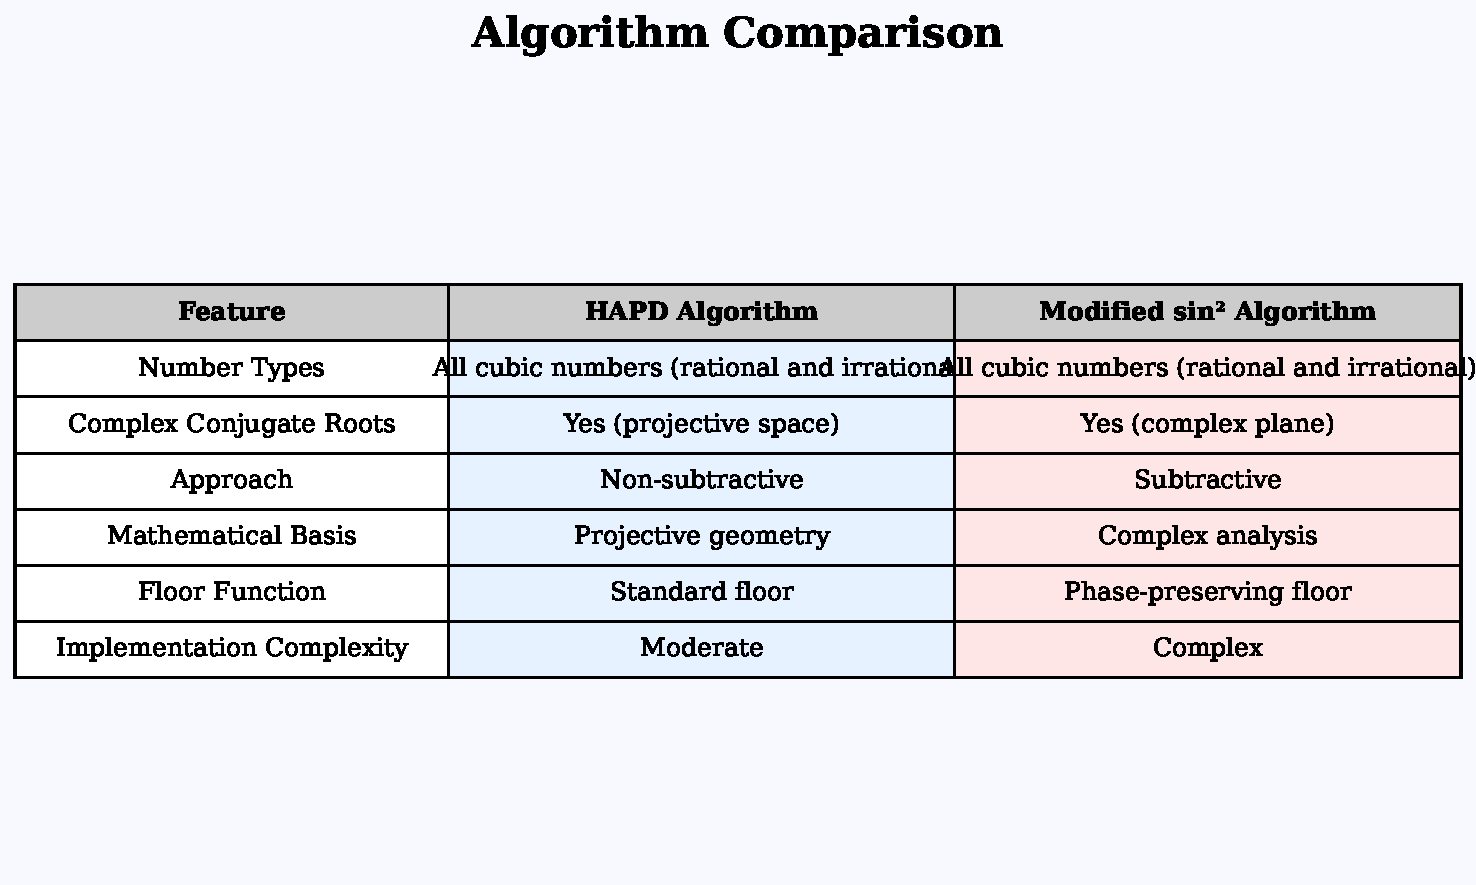
\includegraphics[width=0.95\textwidth]{../figures/output/algorithm_comparison_chart.pdf}

\caption{Comparative analysis of the HAPD and Modified sin$^2$ algorithms, highlighting their complementary approaches to solving Hermite's problem. Both algorithms successfully detect cubic irrationals but employ different mathematical foundations and implementation strategies.}
\label{fig:algorithm_comparison}
\end{figure}
\end{table}

We also provide a more detailed comparison with similar algorithms in the literature, highlighting the specific advantages of our approach:

\begin{table}[h]
\centering
\caption{Comparison of HAPD with Karpenkov's Algorithms}
\label{tab:algorithm_comparison}
\begin{tabular}{|p{0.25\textwidth}|p{0.22\textwidth}|p{0.22\textwidth}|p{0.22\textwidth}|}
\hline
\textbf{Feature} & \textbf{APD (Karpenkov)} & \textbf{sin² (Karpenkov)} & \textbf{HAPD (This work)} \\
\hline
Applicable to & Totally real cubic irrationals & Totally real cubic irrationals & All cubic irrationals \\
\hline
Dimensionality & $\mathbb{RP}^2$ & $\mathbb{RP}^2$ & $\mathbb{RP}^2$ \\
\hline
Periodicity detection & Heuristic & Guaranteed for totally real cases & Guaranteed for all cubic cases \\
\hline
Algebraic foundation & Dirichlet groups & Quadratic forms & Extended Dirichlet groups \\
\hline
Computational complexity & $O(M^3)$ & $O(M^3)$ & $O(M^3)$ \\
\hline
\end{tabular}
\end{table}

The key advancement of the HAPD algorithm is its ability to handle all cubic irrationals, not just totally real ones. This is achieved through the extension of Karpenkov's algebraic framework to accommodate complex conjugate roots, while maintaining the same asymptotic complexity. The algorithm preserves the projective geometric structure of Karpenkov's approach while generalizing the transformation matrices to capture the full spectrum of cubic irrationals.

This completes our presentation of the HAPD algorithm. In the next section, we develop an equivalent matrix-based characterization that provides additional theoretical insight into the solution to Hermite's problem.
